\renewcommand{\contentsname}{Indice}
\tableofcontents
% * PARA MODIFICAR ALGÚN TEMA, HAY QUE IR AL ARCHIVO CORRESPONDIENTE, Y SI SE QUIERE AÑADIR ALGÚN SUB APARTADO, SE AÑADE AHÍ *%
\newpage
\section{Tema 1: Sintaxis y semántica de la lógica proposicional Internet}
\subsection{Cargas}
\noindent La carga es una unidad cuantizable, a partir de la carga del electrón \(e^{-}\),  siendo posible la carga una unidad de magnitud positiva o negativa. \par \noindent
Esta unidad afecta a nivel de la Fuerza Electrostática, el Campo Electrostático y sus magnitudes, y podemos considerar que todas las cargas poseen masa. \par \noindent
Además, dado un sistema, siempre \underline{la suma de todas las cargas va a ser cero}. De este enunciado podemos decir dos principios:


\begin{itemize}
        \item \underline{Principio de Conservación de la Carga}: La suma de todas las cargas del Universo vale cero, es decir, la carga total es \(\bm{cte}\)
        \item \underline{Principio de Conservación local de la Carga}: La suma de todas las cargas en un sistema, es \(\bm{cte}\) es decir, vale 0.
\end{itemize}
\subsection{Ley de Coulumb}
\noindent Esta es la ley fundamental que describe la interacción entre dos cargas puntuales en un medio, independientemente del tamaño del cuerpo. Consideramos la carga total del sistema, y no la unitaria por cada sección del cuerpo. \par
\hspace{4cm}
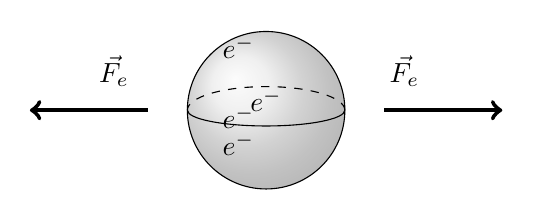
\begin{tikzpicture}
        \shade[ball color = gray!40, opacity = 0.4] (0,0) circle (1cm);
        \draw (0,0) circle (1cm);
        \draw (-1,0) arc (180:360:1 and  0.2);
        \draw[dashed] (1,0) arc (0:180:1 and 0.3);
        \node[left = 10, above = -20]{\(e^-\)};
        \node[left = 0, above = -4]{\(e^-\)};
        \node[left = 10, above = 15]{\(e^-\)};
        \node[left = 10, above = -10]{\(e^-\)};
        \node[right = 50, above = 5]{\(\vec{F_e}\)};
        \draw[->,ultra thick] (1.5,0)--(3,0);
        \node[right = -55, above = 5]{\(\vec{F_e}\)};
        \draw[->,ultra thick] (-1.5,0)--(-3,0);
\end{tikzpicture} \par
\noindent Cada cuerpo generará su propio campo y si consideramos las cargas puntuales, la fuerza entre ambas cargas será:
\[
        \boxed{\vec{F_{12}} = K \hspace{1mm}\frac{q_1q_2}{\left | \vec{r_2} - \vec{r_1} \right |^2}\hspace{2mm}\hat{r} = K \hspace{1mm}\frac{q_1q_2}{\left | \vec{r_2} - \vec{r_1} \right |^3}\hspace{2mm}(\vec{r_2} - \vec{r_1}) \hspace{3mm}N} \hspace{.25cm}
        \substack{\textnormal{\scriptsize{Siendo esta, el vector fuerza que ejerce la carga}} \\
                \textnormal{\(q_1\) sobre la carga \(q_2\).}}
\]
\[
        \boxed{\vec{F_{12}} = -\vec{F_{21}}} \hspace{.25cm}
        \substack{
                \textnormal{\scriptsize{Y evidentemente, el vector fuerza que ejerce la carga \(q_2\) sobre la carga \(q_1\) }}\\
                \textnormal{\scriptsize{es opuesta al vector fuerza que ejerce la carga \(q_1\) sobre la carga \(q_2\)}}
        }
\]
\newline
De esta forma podemos concluir con lo siguiente.
\begin{itemize}
        \item Las cargas de igual signo se repelen, mientras que las de signo diferente se atraen.
        \item Los vectores de posición son respecto a un punto de referencia. Siendo \(\bm{\vec{r_2}}\) el vector del punto destino, y \(\bm{\vec{r_1}}\) el vector del punto de partida.
        \item \(\bm{K}\) es la constante de Couloumb en el vacío y es lo mismo que \(\bm{K = \frac{1}{4\pi\epsilon_{\textnormal{o}}}}\), siendo \(\bm{\epsilon_{\textnormal{o}}}\) la permitividad en el vacío.
\end{itemize}
\subsection{Campo Electrostático}
\noindent El campo es la manifestación de la perturbación en el espacio generado por una carga puntual:
\[
        \boxed{\vec{E} = \hspace{1mm}\frac{\vec{F_e}}{Q} \hspace{1mm}= \hspace{1mm} Kq\frac{\vec{r} -\vec{r`}}{\left | \vec{r} -\vec{r`} \right |^3} \hspace{3mm}V/m} \hspace{1cm}
        \substack{\textnormal{Siendo \(\vec{r`}\) el vector entre el punto de referencia y la carga y }
                \\
                \textnormal{\(\vec{r}\) es el vector entre el punto de estudio y el punto de referencia}
        }
\]
\\
Solo podemos calcular el campo cuando la carga \(\bm{q}\) es muy pequeña, o lo que es lo mismo: \(\bm{\lim_{q \to 0} \vec{E} \approx 0}\) \par
\vspace{0.5cm}
\noindent Sabiendo como se expresa el campo electrostático, nos interesaría conocer algunos casos puntuales dignos de consideración:
\begin{itemize}
        \item Dado un plano con dos cargas puntuales en el mismo eje de coordenadas, y queriendo calcular el campo en un punto cualquiera a una distancia equidistante respecto a las dos cargas es igual a:
              \begin{itemize}
                      \item \(\vec{E_x} = \bm{2\left | \vec{E} \right | \cos{\bm{\alpha}}}\hspace{2mm} \bm{\hat{\imath}}\)
                      \item \(\vec{E_y} = \bm{2\left | \vec{E} \right | \sin{\bm{\alpha}}} \hspace{2mm} \bm{\hat{\jmath}}\)
              \end{itemize}
        \item Las cargas actuan como sumideros.
        \item El campo generado por una carga eléctrica se emite de forma radial y constante, y su número indica su intensidad.
\end{itemize}
\subsection{Distribución de Cargas}
\noindent Hemos considerado un cuerpo cualquiera con carga, como una carga puntual que genera un \(\bm{\vec{E}}\), ya que la carga se distribuía de forma continua. Sin embargo en la realidad no es así, y dependiendo del cuerpo que tengamos, su forma y tamaño afectarán al cálculo del campo. Para esto, deberemos de calcular sección por sección del cuerpo de estudio con el fin de obtener una aproximación del campo total. En esta parte veremos \underline{la distribución de cargas por unidad de longitud} que la denotaremos por:
\[ \boxed{\lambda = \frac{Q}{l}} \hspace{2cm} \textnormal{Siendo \(\bm{Q}\) la carga y \(\bm{l}\) la unidad de longitud}\]
Estudiaremos un caso muy particular, el campo generado por una barra metálica \\ infinítamente larga.\par
\vspace{0.5cm}
\hspace{4.5cm}
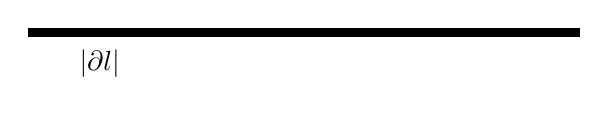
\begin{tikzpicture}
        \node[above = -10, right =15]{\(\left | \partial{l} \right |\)};
        \draw[draw=black, fill=black] (0,0) rectangle ++(7,0.1);
\end{tikzpicture}
\vspace{0.5cm}
\[
        \boxed{\vec{E}(P) \hspace{1mm} = \hspace{1mm}\frac{1}{4\pi\epsilon_o}\int^{b}_{a} \lambda \frac{\hat{r}}{r^2}\hspace{1mm} \mathrm{d}l \hspace{1mm} = K\lambda \int^{b}_{a}\frac{\vec{r}}{r^3} \mathrm{d}l\hspace{1mm} = K\lambda \int_{a}^{b} \frac{y}{h}\vec{\jmath} -\frac{x}{h} \vec{\imath} \hspace{2mm}\mathrm{d}l}
\]
Siendo \(\bm{h = \sqrt[]{x^2+y^2}}\) y las incógnitas \(\bm{x}\) e \(\bm{y}\) como la distancia de un punto cualquiera en la barra para las coordenadas X e Y respectivamente. Los valores \(\bm{a}\) y \(\bm{b}\) de la integral, no son más que dos extremos cualquiera de la barra cargada.
\subsection{Ley de Gauss}
\begin{wrapfigure}{r}{3cm}
        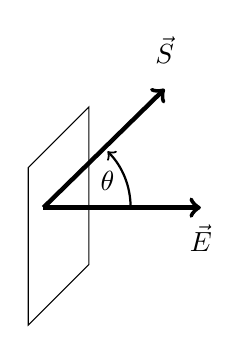
\begin{tikzpicture}[scale=2]
        \pgfmathsetmacro{\cubex}{2}
        \pgfmathsetmacro{\cubey}{1}
        \pgfmathsetmacro{\cubez}{1}
        \draw[] (0,0,0) -- ++(0,0,-\cubez) -- ++(0,-\cubey,0) -- ++(0,0,\cubez) -- cycle;
        \draw[->,ultra thick] (0,-.35,-0.25) --(1,-.35,-.25) node[above = -20]{\(\vec{E}\)};
        \draw[->,ultra thick] (0,-.35,-0.25) -- (30:1) node[above = 5]{\(\vec{S}\)};
        \draw[->,thick] (0.65,-.25) arc (0:45:0.5) node[above = -18]{\( \theta\)};
\end{tikzpicture}
\end{wrapfigure}
\noindent La ley de Gauss define el flujo de \(\bm{\vec{E}}\) a través de una superficie cerrada.\par
\noindent Podemos considerar un caso general, donde dado un espacio cualquiera, con tamaño y forma indefinidos el flujo del campo eléctrico se denota por:
\[
        \phi =\lim_{\Delta S \to 0}\sum_{i=0}^{\infty}\vec{E_i}\hspace{1mm}\Delta S = \int_{S}\vec{E}\hspace{1mm}\mathrm{d} \vec{S} = \boxed{\oint_{S} \vec{E} \hspace{1mm}\mathrm{d} \vec{S} = \frac{Q_\textnormal{int}}{\epsilon_o}}
\]
Dada esta expresión podemos deducir que el flujo total es la suma, infinitesimal de cada una de las secciones sobre la que ejerce el campo eléctrico sobre la superficie, y que el flujo \(\bm{\phi}\) es proporcional a la carga interna \(\Rightarrow \boxed{\bm{\phi} \hspace{1mm} \bm{\alpha} \hspace{1mm} \bm{q}}\) \par
\vspace{1cm}
\hspace{-.5cm}
Por lo tanto podemos estudiar el valor del campo \(\bm{\vec{E}}\) en casos de extrema simetría.
Para esto consideraremos una nueva magnitud \(\bm{\sigma}\) que denota la \underline{distribución superficial de carga}. \(\boxed{\sigma = \frac{Q}{S}}\)
\par \vspace{.5cm} \hspace{-.5cm}No confundir la superficie del cuerpo de estudio con la superficie Gaussiana, esta es variable y depende de quien la estudie.
\subsubsection{Plano Infinito}
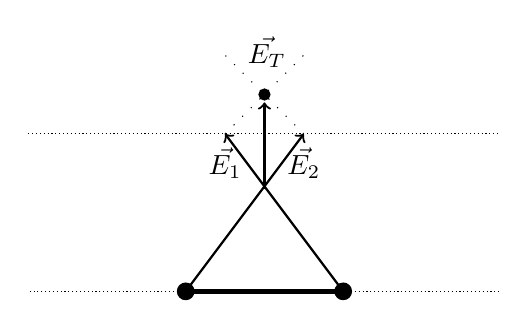
\begin{tikzpicture}
        \draw[densely dotted] (-2,2) -- (4,2);
        \draw[-,ultra thick] (0,0) -- (2,0);
        \draw[densely dotted] (2,0) -- (4,0);
        \draw[densely dotted] (0,0) -- (-2,0);
        \draw[->, thick] (2,0) -- (0.5,2) node[above = -20]{\(\vec{E_1}\)};
        \draw[->, thick] (0,0) -- (1.5,2) node[above = -20]{\(\vec{E_2}\)};
        \filldraw[color = black] (2,0) circle (3pt);
        \filldraw[color = black] (0,0) circle (3pt);
        \draw[loosely dotted] (0.5,2) -- (1.5,3) node[above = 1, left = 3]{\(\vec{E_T}\)};
        \draw[loosely dotted] (1.5,2) -- (0.5,3);
        \filldraw[color = black] (1,2.5) circle (2pt);
        \draw[->, thick] (1,1.3) -- (1,2.4);
\end{tikzpicture}\par
\noindent Dado el diagrama propuesto, todos los puntos situados en el mismo plano, poseen la misma \\Distribución Superficial de Carga, y por ende todos los puntos poseen el mismo
\[\vec{E} = \vec{E_1} + \vec{E_2} = 2\vec{E}\]
\subsubsection{Cilindro en un plano infinito}
\noindent Si situaramos un cilindro en un plano infinitamente largo, observamos que el flujo corresponde a la suma del flujo que pasa por cada una de las tapas y la cubierta lateral del cilindo. De esta forma, debido a que la cubierta lateral es paralela al vector normal al campo, el flujo que pasa por ahí es nulo. Por ende:
\[
        \oint \vec{E}\hspace{1mm}\mathrm{d} \vec{S} = \oint_{SL}\vec{E}\hspace{1mm}\mathrm{d} \vec{S} +\oint_{S^+}\vec{E}\hspace{1mm}\mathrm{d} \vec{S}+\oint_{S^-}\vec{E}\hspace{1mm}\mathrm{d} \vec{S} =
        2 \oint_{S^+} \vec{E}\hspace{1mm}\mathrm{d} \vec{S} \Rightarrow \phi =2\left | \vec{E} \right |\left | \vec{S} \right | = 2ES
\]
\[
        2ES = \frac{Q_{\textnormal{int}}}{\epsilon_o} \Rightarrow E = \frac{\left | \sigma \right |}{2\epsilon_o} \Rightarrow \boxed{\vec{E} = \frac{\sigma}{2\epsilon_o}\hspace{1mm}\hat{n}}
\]
Posteriormente veremos que si el cuerpo está cargado y analizamos el campo \(\bm{\vec{E}}\), este valdrá 0, y por ende su potencial es \(cte\) aunque no sepamos cuanto pueda valer. \textbf{El vector \(\bm{\hat{n}}\) es el vector normal a la superficie}.
\subsubsection{Esfera cargada}
\noindent Aplicando la Ley de Gauss y considerando \(\bm{R}\) el radio de la superficie Gaussiana, y \(\bm{r}\) el radio de la esfera:
\[
        \oint \vec{E} \hspace{1mm} \mathrm{d}\vec{S} \Rightarrow \left | \vec{E} \right | 4\pi R^2 = \hspace{1mm} \frac{Q_{\textnormal{int}}}{\epsilon_o}
\]
\[
        \boxed{\vec{E}  = \hspace{1mm} \frac{Q_{\textnormal{int}}}{\epsilon_o4\pi R^2} \hspace{1mm}\hat{n} \hspace{1mm} = \frac{\sigma r^2}{\epsilon_o R^2} \hspace{1mm}\hat{n}}
\]

\subsection{Balance de Energías}
\begin{wrapfigure}{r}{5cm}
        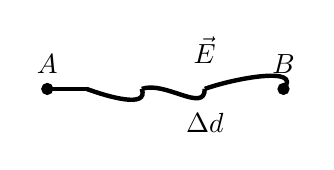
\begin{tikzpicture}
        \draw[-,ultra thick] (0,0) -- (0.5,0);
        \draw[-,ultra thick] (0.5,0) to[out=-20,in=-70] (1.2,0);
        \draw[-,ultra thick] (1.2,0) to[out=20,in=-90] (2,0) node[above =-20]{\(\Delta d\)} node[above =5]{\(\vec{E}\)};
        \draw[-,ultra thick] (2,0) to[out=20,in=50] (3,0);
        \filldraw[color = black] (0,0) circle (2pt) node[above =2]{\(A\)};
        \filldraw[color = black] (3,0) circle (2pt) node[above =2]{\(B\)};
\end{tikzpicture}
\end{wrapfigure}
\noindent ebido a que la fuerza electrostática es una fuerza conservativa, no importa la ruta recorrida, sino las posiciones inicial y final para calcular el trabajo requerido para mover la carga de un punto \textbf{A} al \textbf{B}.\par
\vspace{0.5cm}
\hspace{-.725cm}
De esta forma podemos aplicar \underline{El Teorema de las Fuerzas Vivas} por lo que \(\boxed{W_{A \to B} = \Delta E_c = \frac{1}{2} m (V_B -V_A) \hspace{2mm}J}\)
\par
\vspace{0.5cm}
\hspace{-.6cm}
Por lo tanto el trabajo requerido para mover una carga de un punto A a otro B, es igual a \(\ \Rightarrow \boxed{W_{A \to B} =-\Delta E_p = -q \Delta V}\) \par
\vspace{0.5cm}
\noindent Por convenio diremos que  \(\bm{E_c}\) es la energía cinética, \(\bm{E_p}\) es la energía potencial (ambas en Julios \textbf{J}) y \(\bm{V}\) es el potencial eléctrico, en Vatios \textbf{V}
\[
        \textnormal{En funcion del signo} \rightarrow
        \begin{cases}
                \textnormal{Si \(\bm{W > 0}\), \(\bm{q}\) se mueve a favor del campo} \\
                \\
                \textnormal{Si \(\bm{W < 0}\), \(q\) requiere de un \(\bm{W_{\textnormal{ext}}}\) para moverse.}
                \\
                \textnormal{Si la carga se queda quieta al recorrer ese trayecto, diremos que}
                \\
                \textnormal{\(\bm{W_\textnormal{ext} = -W}\)}
        \end{cases}
\]
\noindent Gracias al conocimiento del trabajo, podemos decir que las unidades del Campo Eléctrico pueden ser tanto \textbf{N/C} como \textbf{V/m}
\subsection{Superficies Equipotenciales}
\noindent Estos son aquellos espacios donde la diferencia de potencial \(\bm{\Delta V}\) vale siempre cero, es decir, tienen el mismo potencial en todos los puntos. \\
Los espacios que satisfacen esta situacion son aquellos situados paralelamente, en sentido del campo eléctrico. \\ Es decir:
\[
        \boxed{\Delta V = - E \mathrm{d} \cos{\alpha} \Rightarrow \mathrm{d}V = - \vec{E}\mathrm{d}\vec{r}}
\]
\begin{wrapfigure}{r}{5cm}
        \begin{tikzpicture}[scale=1]
        \draw[-,thick] (0,0)--(0,3) node[above = -110]{\(V_a\)};
        \draw[-,thick] (3,0)--(3,3) node[above = -110]{\(V_b\)};
        \draw[densely dotted] (-2,1) to[out=20,in=-50] (2,1) node[above = -21]{\(>\)};
        \draw[densely dotted] (2,1) to[out=30,in=10] (3.5,1);
        \draw[densely dotted] (-2,1.75) to[out=20,in=-50] (2,1.75) node[above = -21]{\(>\)};
        \draw[densely dotted] (2,1.75) to[out=30,in=10] (3.5,1.75);
        \draw[densely dotted] (-2,2.5) to[out=20,in=-50] (2,2.5)node[above = -21]{\(>\)};
        \draw[densely dotted] (2,2.5) to[out=30,in=10] (3.5,2.5);
        \node[right = 20, above = 10]{\(\bm{\vec{E}}\)};
\end{tikzpicture}
\end{wrapfigure}
Dada esta expresión, dos puntos son equipotenciales cuando \(\bm{\cos{\bm{\alpha}} = 0}\). Como se puede ver en el diagrama, todos los puntos paralelos, en función de las lineas de cambio, son equipotenciales entre si.
\subsection{Conductores}
\noindent Las cargas en un conductor tenderán a moverse, mientras circula un campo \(\bm{\vec{E}}\), hasta que la carga neta del sistema se estabilice y quede en equilibrio, alrededor de unos \(10^{-14}\) segundos.\\\\
Estos materiales poseen una serie de propiedades, estudiandolos internamente, estas son:\\\\
\hspace{3cm}\textbf{Propiedades:}
\begin{enumerate}
        \item \(\bm{\vec{E}}\) en el interior es nulo, (Si no, las cargas no tenderían a equilibrarse)
        \item  El potencial es \(cte\) en todo el conductor, interior y superficie, es decir, todo el conductor es una superficie equipotencial.
        \item La carga neta tenderá a acumularse en la superficie del conductor, esto se puede demostrar con \underline{la Ley de Gauss}:
              \[
                      \boxed{\oint \vec{E} \mathrm{d} \vec{S} = \frac{Q_{\textnormal{int}}}{\epsilon_{\textnormal{o}}} \Rightarrow \vec{E} = 0 \Leftrightarrow  Q_{\textnormal{int}} = 0}
              \]
        \item El campo \(\bm{\vec{E}}\) en la superficie, hará que la carga se mueva a los bordes, por lo que \(\bm{\vec{E} \not \perp \vec{S}}\)
        \item \(\bm{\vec{E}}\) en la superficie vale \(\bm{\vec{E} = \frac{\sigma}{\epsilon_o}\hat{n}}\)
\end{enumerate}
\vspace{0.5cm}
En la realidad, un conductor no es completamente puro, no siempre, por lo que si este se encontrase en un campo eléctrico externo, \(\bm{\vec{E}}\) interna tenderá a cero, mientras que las cargas internas se moverán a favor del campo externo.
\subsubsection{Jaula de Faraday}
\noindent Son estructuras que son cargadas con carga eléctrica hasta el punto del \underline{Campo de Ruptura}, un estado en el cual el material servirá como aislante frente a campos eléctricos externos.
\subsubsection{Capacidad de un Conductor}
\noindent La expresión de la capacidad \(\bm{\mathcal{C}}\) que se mide en \textbf{Faradios}, \(\bm{F}\), no es más que el cociente entre la carga del sistema entre su potencial:
\[
        \boxed{\mathcal{C} = \frac{Q}{V}}
\]
Esta expresión se consigue a partir de la integración del potencial en un punto de la superficie del conductor, considerando que la \underline{distribución superficial de carga \(\bm{\sigma}\)} es igual al cociente entre la derivada de la carga en función de la superficie. Es decir:
\[
        \sigma = \frac{\mathrm{d}q}{\mathrm{d}S}
\]
\[
        V(p) = \int \frac{\sigma K}{r} \mathrm{d}S \approx Q = V \mathcal{C}
\]
\subsection{Condensador}
\noindent Un condensador es un elemento formado por dos conductores de influencia total, es decir, poseen la misma carga pero de signos distintos. Un caso particular es el condensador de placas planas y paralelas
\newpage
\subsubsection{Condensador de Placas Planas y Paralelas}
\begin{wrapfigure}{l}{0cm}
        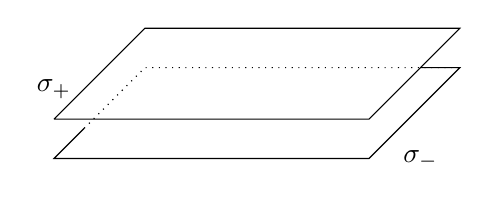
\begin{tikzpicture}{scale = 50em}
        \draw[] (0,0,0) -- (0,0,-3) -- (4,0,-3) -- (4,0,0) -- (0,0,0) node[above = 4]{\(\sigma_+\)};
        \draw[] (0,-.5,-1) -- (0,-.5,0) -- (4,-.5,0) -- (4,-.5,-3) -- (3.5,-.5,-3) node[above = -40]{\(\sigma_-\)};
        \draw[dotted] (0,-.5,-1) -- (0,-.5,-3) -- (4,-.5,-3);
\end{tikzpicture}
\end{wrapfigure}
\noindent Asumiendo que \(\bm{E = \frac{\sigma}{\epsilon_{\textnormal{o}}}}\) es el valor dentro de las dos placas, y \(\bm{d}\) la distancia entre ambas placas, siendo muy pequeña:
\[
        \mathcal{C}  = \frac{Q}{\Delta V} = \frac{Q}{Ed} = \boxed{\frac{\epsilon_{\textnormal{o}S}}{d}}
\]
Posteriormente veremos como, dado un ambiente diferente al vacio, \(\bm{\epsilon_{\textnormal{o}}}\) puede valer otra cosa en función de otra variable.
\subsection{Energía Almacenada en un Condensador}
\noindent Partiendo de que tenemos dos condensadores, uno cargado y otro vacio, ambos con la misma carga pero signos opuestos, las cargas se moverán en función del campo eléctrico que afecta al sistema, redistribuyendo las cargas de forma que cuanta más carga eléctrica se mueva, el potencial eléctrico aumenta proporcionalmente. De esta forma podemos calcular el trabajo, o energía, que se almacena entre las placas:
\[
        \mathrm{d}W = V(q)\mathrm{d}q
\]
\[
        W = \int_{0}^{Q} V(q)\mathrm{d}q = \int_{0}^{Q} \frac{q}{\mathcal{C}}\mathrm{d}q = \frac{q^2}{2\mathcal{C}} \Big|^Q_0 =\frac{Q^2}{2\mathcal{C}}
\]
A veces se denota por la letra \(\bm{\mathcal{\mu}}\), y evidentemente se mide en Julios.
\[
        \boxed{\bm{\mathcal{\mu}} = \frac{Q^2}{2\mathcal{C}} = \mathcal{C}\frac{\Delta V^2}{2}}
\]
Analizandolo de una forma espacial, la energía almacenada no es más que una expresión que relaciona la permitividad del medio y el volumen del campo entre ambas placas:
\[
        \boxed{\bm{\mathcal{\mu}} = E^2 \frac{\epsilon_\textnormal{o}}{2}Sd}
\]
Siendo \(\bm{Sd}\) el volumen entre ambas placas, y \(\bm{\epsilon_\textnormal{o}}\) la permitividad en el vacio, la cual podemos ajustar a cualquier medio.
\subsubsection{Aislantes}
\noindent Al introducir un aislante entre dos placas cualesquiera, \(\bm{\mathcal{C}}\) aumenta, ya que los aislantes se polarizan cuando se someten a un campo eléctrico.\\\\ \textbf{\(\bm{\vec{E}}\) separa las cargas, agrupandolas por su signo y en función de la orientación del propio \(\bm{\vec{E}}\)}
\\\\
Es decir, las cargas se polarizan, en la superficie, y estas tenderán a ser la misma que la polarizada cuanto más cerca estén de la superficie. Pasado un tiempo, la variación de la polarización se invertirá:
\[
        E = \frac{\bm{\sigma_+}-\bm{\sigma_-}}{\epsilon_{\textnormal{o}}}
\]
\subsubsection{Permitivad relativa}
\noindent La permitivad relativa \(\bm{\kappa }\) indica la facilidad con la que la corriente fluye a través de un medio:
\[
        \epsilon_\textnormal{R} = \kappa \epsilon_\textnormal{o}
\]
Siendo \(\bm{\epsilon_\textnormal{R}}\) la permitividad en un medio \(\bm{R}\) y \(\bm{\kappa}\) la permitividad relativa
\subsection{Asociación de condensadores}
\subsubsection{En serie}
\begin{wrapfigure}{r}{6cm}
        \begin{circuitikz}[]
                \draw (-2,0) to[short, l=\(\bm{Q^-}\)] (-1,0)to[C, l_=\(\mathcal{C}\)] (0.5,0)to[short, l=\(0\)] (2,0) to[C, l_=\(\mathcal{C}\)] (3,0) to[short, l=\(\bm{Q^-}\)]  (4,0);
        \end{circuitikz}
\end{wrapfigure}
\noindent \textbf{Por cada uno de los condensadores hay una caida de tensión, pero la intensidad es la misma en todo, por lo que la carga es} \(\bm{cte}\)\\\\
\[
        \boxed{\mathcal{C}_T = \mathcal{C}_{\textnormal{eq}} = \frac{1}{\sum^k_{n=1}\frac{1}{\mathcal{C}_n}}}
\]
\[
        \boxed{V_T = \sum^n_{i=1}V_n}
\]
\[
        \boxed{Q_n = Q_1 = ... = Q_k = cte}
\]

\subsubsection{En paralelo}
\begin{wrapfigure}{r}{1cm}
        \begin{circuitikz}
                \draw (0,0) to[C=\(\mathcal{C}\)] (2,0);
                \draw (0,-2) to[C=\(\mathcal{C}\)] (2,-2);
                \draw (0,-4)  to[C=\(\mathcal{C}\)] (2,-4);
                \draw (0,0)--(0,-6) (2,0)--(2,-6);
        \end{circuitikz}
\end{wrapfigure}
\noindent \textbf{Por cada uno de los condensadores la tensión es la misma, es \(\bm{cte}\), pero la carga no, por lo que la intensidad depende de cada capacitor}:
\[
        \boxed{\mathcal{C}_T = \mathcal{C}_\textnormal{eq} = \sum^k_{n=1}\mathcal{C}_n}
\]
\[
        \boxed{V_n = V_1 = ... = V_k = cte}
\]
\[
        \boxed{Q_T = \sum^k_{n=1}Q_n}
\]
\newpage
\section{Tema 2: Deducción natural proposicional}
\subsection{Congruencia}
\noindent Considerando un número \(\mathbf{n}\), que diremos que se comporta como 0 en un sistema \(\mathbb{Z}_n\). De esta forma definimos una función tal que:
\[
        y - x = nk
\]
\noindent El primer miembro es congruente con cualquier múltiplo \(k\) de \(n\)\\ Esto se representa como:
\[
        \boxed{a \equiv b(\textnormal{mod}\hspace{2mm}n)}
\]
\noindent De esta forma, el rango posibles de valores, son \(\mathbf{n} = {0,...,n-1}\).\par
\noindent\fbox{{\large Propiedades}} \par
\begin{itemize}
        \item Equivalencia. Teniendo dos congruencias de este tipo:\[\begin{cases}
                              \mathbf{a \equiv b(\textnormal{\textbf{mod}}\hspace{2mm}n)}\\ \mathbf{b \equiv c(\textnormal{\textbf{mod}}\hspace{2mm}n)}\end{cases}\]\noindent Entonces: \[\boxed{\mathbf{a \equiv c(\textnormal{\textbf{mod}}\hspace{2mm}n)}}\]
        \item No existen divisiones por cero, por lo que \(ab \not \Rightarrow a = 0 \textnormal{\hspace{5mm}ó\hspace{5mm}} b = 0\)
        \item Si existe un \(\lambda \in \mathbb{Z}\) entonces:\[\begin{cases}
                              \mathbf{a \equiv b(\textnormal{\textbf{mod}}\hspace{2mm}\lambda n)}\\ \mathbf{\lambda a \equiv \lambda b(\textnormal{\textbf{mod}}\hspace{2mm}\lambda n)}\end{cases}\] \noindent Será siempre igual a\(a \equiv b(\textnormal{mod}\hspace{2mm}n)\), solo si \(\lambda \neq 0\).
        \item Sumar, restar o multiplicar dos congruencias del mismo modulo, será lo mismo que una congruencia, con los terminos \(a\) y \(b\) iguales a sumar, resta o multiplicar en ambas congruencias.
\end{itemize}
\subsection{Inversas}
\noindent Existe un modulo inverso cuando existe un único resultado a la ecuación \(\boxed{\mathbf{{a\mathrm{X} = 1}}}\) con \(\mathbf{a \in \mathbb{Z}_n}\)
\subsubsection{Calculo de Inversas}
\noindent Es un proceso muy simple.\\ Planteamos una ecuación de congruencia:
\[
        a\mathrm{X} = 1 (\textnormal{mod}\hspace{2mm}n)
\]
\noindent Si la convertimos a una \underline{ecuación diofantica}, podemos calcular el coeficiente de la identidad de \underline{Bezout} correspondiente al termino \(\mathrm{X}\).
\[
        a\mathrm{X} - n\mathrm{Y} = 1
\]
Tras resolverlo, obtendremos un \(\alpha\) que al calcular su resto respecto a \(n\), obtendremos el inverso \(\mathbf{a^-1}\).\par
\noindent Podemos expresar entonces el calculo del inverso de la siguiente forma:
\[
        \boxed{1 \equiv (\alpha (\textnormal{mod}\hspace{2mm}n))(\textnormal{mod}\hspace{2mm}n)}
\]
\subsection{Ecuaciones en Congruencias}
\noindent Partiendo de una congruencia como la vista al principio del tema:
\[
        \boxed{a \equiv b(\textnormal{mod}\hspace{2mm}n)}
\]
\noindent Toda ecuación en congruencia se puede resolver como una ecuación diofantica.
\subsubsection{Sistemas de Ecuaciones en Congruencias, Teorema Chino del Resto}
\subsection{Función de Euler}
\noindent Dado una función \(\mathbf{\phi (N)}\), que nos indicará el numero de elementos en base \(N\) que tienen inverso, podemos calcular los valores en base a las siguientes indicaciones:
\begin{itemize}
        \item Si \(N \in \mathbb{P}\), es decir, \(N\) es primo: \(\boxed{\mathbf{\phi (N) = N - 1}}\)
        \item Si \(N\) es primo y está elevado a un número \(m\):\(\boxed{\mathbf{\phi (N^m) = N^{m-1}(N-1)}}\)
        \item Si \(N\) lo podemos descomponer en factores primos, entonces \(\boxed{\mathbf{\phi (N) = \phi(A)\hspace{5mm} \phi(B)}}\)
\end{itemize}
\noindent De esta forma nos quedarán dos expresiones para calcular \(\phi(N)\):
\[
        \phi(N) = n \prod^k_{n=t}(1-p_n^{-1})
\]
\[
        \boxed{\phi(N)   = \prod^k_{n=t}(p_n^{m_n-1})(p_n-1)}
\]
\noindent Siendo \(p_n\) los factores primos del número en cuestión y \(m_n\) el numero de veces que aparece ese factor primo en cuestión.
\subsection{Teoremas}
\noindent Aquí veremos dos teoremas que nos ayudarán a extraer propiedades y conclusiones para temas posteriores.
\subsubsection{Teorema de Fermat}
\noindent Sabemos por definición que dado un conjunto \(\mathbb{Z}_n\), no pueden haber elementos repetidos y que existen \(n-1\) elementos. De esta forma enunciamos:
\par \noindent Si \(\mathbf{p}\) es primo, \(\mathbf{x>0}\) y \(\mathbf{p\not |\hspace{3mm}x }\) entonces:
\[
        \boxed{x^{p-1} \equiv 1(\textnormal{mod}\hspace{2mm}p)}
\]
\noindent Si solo ocurriese que \(\mathbf{p}\) es primo y \(\mathbf{x>0}\):
\[
        \boxed{x^{p} \equiv x(\textnormal{mod}\hspace{2mm}p)}
\]
\subsubsection{Teorema de Euler}
\noindent Es una ramificación del \underline{Teorema de Fermat}, y dice que si \(x\) y \(n\) son coprimos entonces:
\[
        \boxed{x^{\phi(n)} \equiv 1(\textnormal{mod}\hspace{2mm}n)}
\]
\subsubsection{Potencias de Fermat}
\noindent Esta es una forma rápida de convertir una potencia a otra, en una congruencia específica:
\[
        x^k\hspace{1mm}\textnormal{mod}\hspace{2mm}p = x^{(p-1)\left \lfloor \frac{k}{p-1} \right \rfloor + k\hspace{1mm}\textnormal{mod}\hspace{2mm}(p-1)}=\boxed{x^{k\hspace{1mm}\textnormal{mod}\hspace{2mm}(p-1)}\textnormal{mod}\hspace{2mm}p}
\]
\subsection{Metodo MC, potencias rapidas}
\subsection{Criptografía y RSA}

\newpage
\section{Tema 3: Tableros semánticos proposicionales}

\subsection{Intensidad de Corriente}
\begin{wrapfigure}{r}{3cm}
        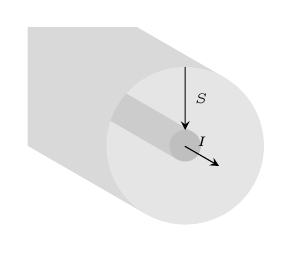
\begin{tikzpicture}
                \clip (-2,-1.1) rectangle (1,1.5);
                \begin{scope}[rotate=-30]
                        \fill[gray!30] (-3,-1) rectangle (0,1);
                        \fill[gray!20] (0,0) circle(1cm);
                        \begin{scope}
                                \clip(0,0) circle(1cm);
                                \fill[gray!40] (-3,-0.2) rectangle (0,0.2);
                                \fill[gray!50] (0,0) circle(2mm);
                        \end{scope}
                        \draw[-stealth] (120:1) -- node[right,font=\tiny]{$S$}(120:0.2);
                        \draw[-stealth] ([yshift=-0.5\pgflinewidth]0,0) -- node[above,font=\tiny]{$I$}([yshift=-0.5\pgflinewidth]0.5,0);
                \end{scope}
        \end{tikzpicture}
\end{wrapfigure}
\noindent Definimos la Intensidad como la cantidad de corriente que circula por una sección de un conductor:
\[
        I \hspace{1mm}= \hspace{1mm} \frac{\mathrm{d}q }{\mathrm{d} t}
\]
\noindent De esta fórmula podemos también obtener los valores de \(\mathbf{d}\bm{q}\) y por ende \textbf{I}:
\[
        \boxed{\mathrm{d}q \hspace{1mm}= \hspace{1mm} n\hspace{.5mm}\left | q\right |\hspace{.5mm}v_d\hspace{.5mm}S\hspace{.5mm}\mathrm{d}t}
\]
\[
        \boxed{I \hspace{1mm}= \hspace{1mm} n\hspace{.5mm}\left | q\right |\hspace{.5mm}v_d\hspace{.5mm}S\hspace{.5mm}}
\]
Siendo las incógnitas:
\begin{itemize}
        \item \(\bm{n}\): Es el número de cargas que fluyen por unidad de volumen \textbf{C/V}.
        \item \(\bm{v_d}\): Es la velocidad de deriva con que se mueven las cargas \textbf{m/s}.
        \item \(\bm{S}\): Es la sección transversal, su superficie.
        \item \(\bm{q}\): Es el valor de la carga que circula, tomaremos en un principio valores positivos, es decir en valor absoluto.
\end{itemize}
\subsection{Vector Densidad de Corriente}
\noindent Esta es una magnitud vectorial con la cual podemos medir la intensidad que atraviesa una superficie:
\[
        I \hspace{1mm} = \hspace{1mm} \int_{S} \vec{J}\hspace{3mm}\mathrm{d}\hspace{.5mm}\vec{S}\hspace{3mm}\Rightarrow  \boxed{J\hspace{1mm} = \hspace{1mm} \left | \frac{I}{S} \right |}
\]
\subsubsection{Campo Electrostático y Densidad de Corriente}
\noindent Entre \(\bm{\vec{J}}\) y \(\bm{\vec{E}}\) existe una relación muy estrecha, y es que cuanto \(\bm{\vec{E}}\) aumenta, debido a que \(\bm{v_d}\) se incrementa, \(\bm{\vec{J}}\) crece proporcionalmente:
\[
        \bm{\vec{J}} \hspace{2mm} \bm{\propto} \hspace{2mm} \bm{\vec{E}}
\]
\subsection{Conductores Ohmicos}
\noindent Conocemos ya dos conceptos que nos permitirán deducir la resistividad que posee un material, el \underline{Campo Eléctrostático} y la \underline{Densidad de Corriente}, además de la Ley de Ohm \(\bm{V = IR}\), que relaciona la Tensión con la Resistencia y la Intensidad:
\[
        \boxed{\vec{J} \hspace{1mm} = \hspace{1mm} \sigma \vec{E}}
\]
\[
        \boxed{\vec{E} \hspace{1mm} = \hspace{1mm} \rho \vec{J}}
\]
Siendo \(\bm{\sigma}\) la \underline{Conductividad Eléctrica} en \underline{Siemens} entre metros \textbf{S/m} y \(\bm{\rho}\) la \underline{Resistividad Eléctrica} en ohmios por metro \(\bm{\omega}\)\textbf{m}
\subsubsection{Resistencia}
\noindent Considerando que la caída de tensión entre los extremos de una resistencia vale \\ \(\bm{\Delta V_{\textnormal{ba}}} \hspace{1mm}= \hspace{1mm} \bm{V_\textnormal{b}} -\bm{V_\textnormal{a}}  \Rightarrow \bm{\Delta V_{\textnormal{ba}}}\hspace{1mm}= \hspace{1mm} \bm{E \mathrm{d}l}\) y teniendo en cuenta la definición de \(\bm{\vec{J}}\) podemos concluir en lo siguiente:
\[
        \boxed{\bm{\frac{V}{I} = \frac{E\mathrm{d}l}{\sigma E S} = \frac{\mathrm{d}l}{\sigma S} = \frac{\rho \mathrm{d}l}{S} = R = cte}}
\]
\subsection{Joule}
\noindent Este es un efecto, que se produce en una resistencia, que define que hay una disipación de la energía en forma de calor, ya que al pasar por una resistencia, la tensión que sale \(\bm{V_b}\) es menor que la que entra \(\bm{V_a}\):
\[
        \mathrm{d}Q \hspace{1mm} = \hspace{1mm} cte \hspace{1mm} = \hspace{1mm} I
\]
\[
        \mathrm{d}V \hspace{1mm} = \hspace{1mm} \mathrm{d}Q \Delta V_{\textnormal{ba}}\]
\[
        -\frac{\mathrm{d} v}{\mathrm{d} t} \hspace{1mm} = \hspace{1mm} \frac{\mathrm{d} Q}{\mathrm{d} t}\Delta V_{\textnormal{ab}} \hspace{1mm} = \boxed{P_{\textnormal{disipada}} \hspace{1mm} = \hspace{1mm} V I \textnormal{[\textbf{W}]}}
\]
\subsection{Baterías}
\noindent Las baterías están formadas por un generador interno y una resistencia en serie, este generador produce una f.e.m (\(\bm{\varepsilon}\)). Idealmente:
\[
        W \hspace{1mm} = \hspace{1mm} \Delta U \hspace{1mm} = \hspace{1mm} \Delta QV
\]
\[
        \varepsilon \hspace{1mm} = \hspace{1mm} \frac{W}{\Delta Q} \hspace{1mm} = \hspace{1mm} V
\]
Es decir: \(\boxed{\bm{P_{\textnormal{suministrada}}} \hspace{1mm} = \hspace{1mm} \bm{\varepsilon I - I^2r}}\) en una situación ideal \(\bm{r}=\)0\(\bm{\Omega}\)
\subsection{Leyes de Kirchoff}
\noindent Se aplica a circuitos que no se pueden resolver aplicando las leyes de Ohm solamente, se basa en el uso de mallas que dividen la corriente y su sentido, en función de la orientación de las pilas
\subsubsection{Leyes de los Nudos}
\begin{wrapfigure}{r}{3cm}
        \begin{tikzpicture}
                \draw[->] (-2,0) -- (-1, 0) node[above = 1]{\(\bm{I_1}\)};
                \draw[-] (-1, 0) -- (0, 0);
                \draw[->] (0,0) -- (1,0) node[above = 1]{\(\bm{I_4}\)};
                \draw[->] (0,0) -- (1,-1.2) node[above = 1]{\(\bm{I_2}\)};
                \draw[->] (0,0) -- (1, 1.3) node[above = 1]{\(\bm{I_3}\)};
                \draw[-] (1,0) -- (2,0);
                \draw[-] (1,-1.2) -- (2,-1.2);
                \draw[-] (1, 1.3) -- (2, 1.3);
        \end{tikzpicture}
\end{wrapfigure}
\noindent También conocida como \textbf{LCK}, define, como aparece en el esquema, que la intensidad que circula por un circuito, es igual a la suma de todas aquellas intensidades que se generan al pasar por un nodo y bifurcarse. Se define como:
\[
        \boxed{I_T \hspace{1mm} = \hspace{1mm} \sum_{n=1}I_n}
\]
\subsubsection{Leyes de las Mayas}
\noindent También conocida como \textbf{LTK} define que la suma de todas las tensiones de cada malla debe ser igual a cero:
\[
        \boxed{\sum_{n=1}V_n \hspace{1mm} = \hspace{1mm} 0\textnormal{\textbf{V}}}
\]
\noindent Por defecto consideraremos que si la corriente va del polo positivo al negativo de la pila, tiene sentido negativo, y positivo en el contrario. Esta misma regla se aplicará a las resistencias.
Las resistencias de una misma corriente se sumarán, y en función del sentido de la corriente con la que puedan coincidir, se sumarán si van en el mismo sentido.
\subsubsection{Circuitos simples y Paralelos}
\subsubsection{Simples}
\begin{itemize}
        \item Tensión: La tensión total es la suma de todas las tensiones.
        \item Intensidad: es \textbf{cte}.
        \item Resistencia: La resistencia total es la suma de todas las resistencias.
\end{itemize}
\subsubsection{Paralelos}
\begin{itemize}
        \item Tensión: Es \textbf{cte} porque la carga es la misma en cada rama.
        \item Intensidad: La intensidad total es la suma de todas las intensidades.
        \item Resistencia: La resistencia total es la suma de todas las resistencias, inversas, y nuevamente inversa: \(\bm{\frac{1}{R_T} = \sum_{n = 1}\frac{1}{R_n}}\)
\end{itemize}
\subsection{Transistores}
\begin{wrapfigure}{l}{0cm}
        \begin{tikzpicture}
                \path (0,0) coordinate (ref_gnd);
                \draw
                (ref_gnd)
                to[battery=\(V\)] ++(0,1)
                to[nos] ++(0,2)
                to[R=\(R\)] ++(3,0)
                to[C=\(C\)] ++(0,-3)
                -- (ref_gnd);
        \end{tikzpicture}
\end{wrapfigure}
\noindent El circuito de la figura es un circuito RC, es decir, posee una resistencia y un condensador.
Vamos a estudiar este circuito para dos momentos concretos en el tiempo, en el instante inicial y cuando ha transcurrido mucho tiempo, indefinido.
\vspace{.5cm}
\par \noindent Cuando el circuito se enciende por primera vez, \(\bm{t = 0}\) en el instante en el que se pulsa el interruptor, la intensidad que circula por el circuito es la misma en todo momento, ya que \underline{el condensador está vacío y actúa como un cable}.
\vspace{.5cm}
\par \hspace{-0.5cm}Cuando ha pasado un tiempo indefinido \(\bm{t \rightarrow \infty}\), deja de circular corriente porque \underline{el condensador se ha cargado y ahora funciona como un cable}\\
\underline{roto, hay cortocircuito}.
\\
\\
\noindent Ecuaciones:
\begin{itemize}
        \item \(\bm{Q(t)=Q_f(1-e^{-\frac{t}{RC}})}\)
        \item \(\bm{I(t)=\frac{\varepsilon}{R}e^{-\frac{t}{RC}}}\)
        \item \(\bm{V_R(t) = \varepsilon e^{-\frac{t}{RC}}}\)
        \item \(\bm{V_C(t) = \varepsilon(1-e^{-\frac{t}{RC}})}\)
\end{itemize}

\newpage
\section{Tema 4: Formas Normales}
\subsection{Introducción}
\subsection{Descripción General}
\subsection{Arquitectura Interna}
\subsection{Organización de la Memoria}
\subsection{Modos de Direccionamiento}
\subsection{Juego de Instrucciones}
\subsection{Directivas de Ensamblador}
\newpage
\section{Tema 5: Resolución proposicional}
\subsection{Uso de fasores}
\noindent Debido a que los cálculos con números complejos pueden llegar a ser complicados, es más propicio usar fasores en este tema. El fasor más simple que podemos calcular, de temas anteriores, se puede obtener para calcular la tensión inducida de una espira.
\[
        \varepsilon (t) = -\frac{\mathrm{d} \Phi}{\mathrm{d} t} = -\left | \vec{B} \right |\left | \vec{S} \right |\frac{\mathrm{d} \cos{(wt+\rho )}}{\mathrm{d} t} = \varepsilon_{\textnormal{o}}\sin{(wt + \rho)}
\]
\noindent Normalmente, la amplitud se refleja con valores eficaces \(\mathbf{X_{\textnormal{e}} = \frac{X_{\textnormal{o}}}{\sqrt{2}}}\).
\subsection{Impedancia}
\noindent La impedancia es la forma de representar la ''resistencia"\space que oponen los elementos de un circuito de corriente continua al paso de la corriente.\\
Dependiendo del elemento, resistencia; bobina o capacitor, la señal estará en fase o desfase.\\ Se miden en ohmios.
\begin{itemize}
        \item Resistencias:
              \(\boxed{\mathbf{R = \frac{\tilde{V}}{\tilde{I}}}}\) Se encuentra en resonancia, misma fase.
        \item Condensadores:
              \(\boxed{\mathbf{\mathrm{C} = \frac{\tilde{I}}{w\tilde{V}j} \Rightarrow X_{\mathrm{C}} = \frac{-j}{w\mathrm{C}}}}\) Se encuentra en desfase, de \(\mathbf{-\frac{\pi}{2}}\).
        \item Bobinas:
              \(\boxed{\mathbf{L = \frac{\tilde{V}}{w\tilde{I}j} \Rightarrow X_L =jwL}}\) Se encuentra en fase, de \(\mathbf{\frac{\pi}{2}}\)
\end{itemize}
La suma de impedancias sigue la misma regla que la suma de resistencias \[
        \boxed{Z_T = \underset{\textnormal{serie}}{\sum_{n=1}^{k} Z_n} = \underset{\textnormal{paralelo}}{\frac{1}{\sum_{n=1}^{k}\frac{1}{Z_n}}}}
\]
\subsection{Potencia}
\noindent Aquí solo veremos las fórmulas correspondientes:
\begin{itemize}
        \item \(
              \boxed{P(t) = \tilde{V}\tilde{I} = V_{\textnormal{o}}\cos{(wt + \rho)}\hspace{3mm}I_{\textnormal{o}}\cos{(wt)}} \hspace{5mm} \) Esta es la expresión general para calcular la potencia que consume, o el calor que se pierde en el circuito.
        \item \(
              \boxed{P_m = \frac{V_{\textnormal{o}}I_{\textnormal{o}}\cos{\rho}}{2}}\hspace{5mm}
              \) De aquí podemos deducir la potencia que consume el circuito en total, siendo \(\mathbf{\rho = \rho_v - \rho_I}\).
        \item \(
              \boxed{P_R= \frac{V_{\textnormal{o}}I_{\textnormal{o}}}{2}\hspace{5mm}}\) Aquí vemos que la potencia consumida por \underline{las resistencias} es igual que en un circuito de corriente continua.
              \item\(\boxed{P_z = \frac{I_{\textnormal{o}}^2}{2}\hspace{2mm} \Re(z) = O} \hspace{5mm}
              \) Todo lo que no sea una resistencia, no consumirá energía, por lo que su potencia es siempre 0.
\end{itemize}
\subsection{Ondas en un circuito}
\noindent Este es un caso especial, que aparece en las telecomunicaciones, veremos las ecuaciones más relevantes, unicamente:
\[
        \tilde{\varepsilon} = \tilde{I}Z
\]
\[
        \boxed{I_{\textnormal{o}} = \frac{\varepsilon_{\textnormal{o}}}{\sqrt{R^2+(X_L - X_C)^2}}}
\]
\noindent Cuando \(\mathbf{X_L = X_C}\) entonces decimos que están en resonancia y podremos calcular la frecuencia:
\[
        \boxed{Lw_{\textnormal{o}} = \frac{1}{\mathrm{C}w_{\textnormal{o}}}}
\]
\[
        f_{\textnormal{o}} = \frac{1}{2\pi\sqrt{L\mathrm{C}}}
\]
\noindent Y por ende:
\[
        \boxed{\tilde{V_L} = -\tilde{V_C}}
\]
\begin{wrapfigure}{l}{2cm}
        \begin{tikzpicture}
                \path (0,0) coordinate (ref_gnd);
                \draw
                (ref_gnd)
                to[battery=\(\varepsilon\)] ++(0,1)
                to[nos] ++(0,2)
                to[R=\(R\)] ++(3,0)
                to[L=\(L\)] ++(0,-3)
                to[C=\(\mathrm{C}\)] ++ (-3,0)
                -- (ref_gnd);
        \end{tikzpicture}
\end{wrapfigure}
\noindent Aquí vemos un dibujo del circuito que estamos analizando:
\newpage
\section{Tema 6: Algoritmos para SAT. Aplicaciones}
\subsection{Introducción}
\subsection{Limite con dos variables}
\subsubsection{Continuidad}
\subsection{Diferenciabilidad}
\subsubsection{Primer Orden}
\subsubsection{Segundo Orden}
\subsubsection{Diferenciales Cruzadas}
\subsection{Diferenciabilidad en un punto}
\subsection{Vector Gradiente}
\subsection{Derivada Direccional}
\subsection{Condición Suficiente de Diferenciabilidad}
\subsection{Condición Necesaria de Diferenciabilidad}
\subsection{Plano Tangente}
\subsection{Extremos Relativos}
\noindent Calculamos las derivadas parciales de primer orden de la función y obtenemos con que valores ambas se anulan:
\[
        \frac{\partial f(x,y)}{\partial x} = 0 \hspace{0.75cm},\hspace{0.75cm} \frac{\partial f(x,y)}{\partial y} = 0
\]
\noindent De aquí obtendremos un conjunto \(\phi = \left \{ \left.  x_0, y_0, ... x_n, y_n\right \} \right.\)\par \noindent Tras esto construiremos una matriz Hessiana, formada por las derivadas parciales de segundo orden, y calcularemos su determinante:
\[\boxed{HF(x,y) = \begin{pmatrix}
                        \frac{\partial f(x,y)}{\partial^2 x}           & \frac{\partial f(x,y)}{\partial x \partial y} \\
                        \frac{\partial f(x,y)}{ \partial y \partial x} & \frac{\partial f(x,y)}{\partial^2 y}
                \end{pmatrix}}
\]
\[
        |HF(x,y)| =  \frac{\partial f(x,y)}{\partial^2 x} \frac{\partial f(x,y)}{\partial^2 y} - \frac{\partial f(x,y)}{\partial x \partial y}\frac{\partial f(x,y)}{ \partial y \partial x} = \Delta
\]
\noindent Tras obtener este determinante, sustituye \(x\) e \(y\) por los valores obtenidos previamente. De esta forma llegaremos a 4 conclusiones:
\[
        \Delta
        \begin{cases}
                \Delta = 0 \text{\hspace{1cm}No hay información suficiente para indicar si es un Punto Crítico}
                \\
                \Delta \neq 0
                \begin{cases}
                        \Delta < 0  \text{\hspace{1cm}Punto de Silla}
                        \\
                        \Delta > 0
                        \begin{cases}
                                \frac{\partial f(x,y)}{\partial^2 x} < 0  \text{\hspace{1cm}Es un máximo relativo}
                                \\
                                \frac{\partial f(x,y)}{\partial^2 x} > 0  \text{\hspace{1cm}Es un mínimo relativo}
                        \end{cases}
                \end{cases}
        \end{cases}
\]
\newpage
\section{Tema 7: Sintaxis y semántica de la lógica de primer orden}
\subsection{Sintaxis}
\noindent Aprovecharemos toda la sintaxis dada en la \textit{Lógica Proposicional} más nuevas formas de representar el conocimiento, siendo más parecidas al lenguaje natural.
\subsubsection{Nuevos Elementos}
\noindent Representaremos nuestros entornos con 4 términos posibles:
\begin{itemize}
        \item \textbf{Constantes}: Objetos de nuestro entorno, cuyo valor es fijo. Ej: \((a,b,c,...\)
        \item \textbf{Variables}: Objetos de nuestro entorno los cuales pueden representar cualquier objeto de nuestro dominio del problema. Ej: \(x,y,z,...\)
        \item \textbf{Predicados}: Un tipo de expresión, que recibirá de 0 a N parámetros objeto, indicado por su \textit{aridad}, y el cual devolverá o verdadero o falso. Se representan con la letra mayúscula
        \item \textbf{Funciones}: Expresiones las cuales reciben objetos y devuelven otro objeto. Se representan con la letra minúscula.
\end{itemize}
\subsubsection{Nuevos Símbolos}
\begin{itemize}
        \item \(\forall\): Es un cuantificador universal, que indica que verifica la condición para cualquier objeto del dominio del problema.
        \item \(\exists\): Es un cuantificador existencial, que indica que la condición se verifica para al menos 1 elemento de nuestro dominio del problema.
        \item \(=\): Es un operador que compara dos objetos.
\end{itemize}
\subsection{Variables Libres o Ligadas}
\noindent Denominamos a estas variables a aquellas tales que dada una expresión, serán \textbf{libres} si aparece fuera de un operador cuantificador una vez, y \textbf{ligadas} si aparece dentro de uno.
\[\forall_x (P(x) \rightarrow R(x,y))\]
\noindent \(x\) es ligada mientras que \(y\) es libre.

\subsection{Estructura del Lenguaje}
\noindent Una estructura del lenguaje es un par \textbf{Universo}, \textbf{Interpretación}, lo representamos así:
\[\mathbb{I} = (U, \mathrm{I})\]
\begin{itemize}
        \item Denominamos \textbf{Universo} al conjunto de objetos que conforman nuestro dominio del problema.
        \item Denominamos \textbf{Interpretación} al conjunto de constantes, funciones y predicados que usaremos sobre el Universo.
\end{itemize}
\[
        \mathbb{I} = (\left \{ u,v,w \right \}, \left \{ (b,c),(P/1,Q/2),(f/2) \right \})
\]
\noindent Con estas dos herramientas, Universo e Interpretación, podremos obtener modelos de una expresión aplicando las interpretaciones a cada operador de la expresión, usando como objetos del problema los objetos del universo.
\par\noindent Diremos que una \textbf{estructura} e \textbf{interpretación} es una realización de \(F\) tal que la expresión tiene modelo con esa interpretación.
\par \noindent La \textbf{estructura} es un modelo de \(F\) cuando para toda interpretación de la estructura, \(F\) es un modelo.
\newpage
\section{Tema 8: Deducción Natural en lógica de primer orden}
\subsection{Sustituciones}
\noindent Definimos una \textit{sustitución} \(\sigma \) a la aplicación de un objeto \(t\) a un término de nuestro Universo.
\par \noindent Los podemos definir de la siguiente forma:
\[
        \boxed{F\left [ x_1 / t_1, ..., x_n / t_n \right ]}
\]
\noindent Siendo \(F\) el término a evaluar, y \(x_n / t_n\) la sustitución del objeto \(x_n\) por el \(t_n\).
\par \noindent Un ejemplo es el siguiente:
\[\sigma = \left [ x / f(y),  y/b \right ]\]
\[A \equiv \forall_x (Q(x) \rightarrow R(x,y)) = \forall_x (Q(x) \rightarrow R(x,b))\]
\[B \equiv Q(x) \rightarrow \forall_x R(x,y) = Q(f(y)) \rightarrow R(x,b)\]
\noindent \textbf{Son fórmulas resultantes de una sustitución de \textit{ocurrencias libres}}.
\subsubsection{Sustituciones Libres}
\noindent Esta clase de sustituciones no introducen ninguna  ocurrencia nueva, de ninguna variable. Un ejemplo de una que no lo es:
\[\exists_x (x < y) =_{\left [ y/x \right ]} \exists_x(x<x)\]
\subsection{Reglas de Deducción Natural de Cuantificadores}
\noindent Vamos a aprovechar todas las reglas anteriores para esto, más unas pocas más:
\subsubsection{Regla del Cuantificador Universal Introducción}
\[
        \boxed{\frac{\boxed{\begin{matrix}
                                        x_o \hspace{2mm}\text{supuesto} \\
                                        \vdots                          \\
                                        F\left [ x/x \right ]
                                \end{matrix}}}{\forall_x F} \hspace{2mm} \forall i}
\]
\subsubsection{Reglas del Cuantificador Existencial Introducción}
\[
        \boxed{\frac{F\left [ x/t \right ]}{\exists_xF} \hspace{2mm} \exists i}
\]
\subsubsection{Regla del Cuantificador Universal Eliminación}
\[
        \boxed{\frac{\forall_x F}{F\left [ x/t \right ]} \hspace{2mm} \forall e
        }\]
\subsubsection{Reglas del Cuantificador Existencial Eliminación}
\[
        \boxed{\frac{\exists_x F\hspace{2mm}\boxed{\begin{matrix}
                                        x_o \hspace{2mm}\text{supuesto} \\
                                        \vdots                          \\
                                        G
                                \end{matrix}}}{G} \hspace{2mm} \exists e}
\]
\subsubsection{Ejemplos}
\[\left \{ \forall_x(P(x)\rightarrow Q(x)) \right \}
        \models \forall_x P(x) \rightarrow \forall_xQ(x)
\]
\[
        \boxed{\begin{matrix}
                        1)\hspace{2mm} \forall_x(P(x)\rightarrow Q(x)) \hspace{5mm} \text{Premisa}             \\
                        \hspace{2mm}2)\hspace{2mm} \forall_x P(x) \hspace{24mm} \text{Supuesto}                \\
                        3) x_0 \hspace{33mm} \text{Supuesto}                                                   \\
                        \hspace{-30mm}4)P(x_0) \hspace{5mm} \forall e \hspace{2mm} 2                           \\
                        \hspace{-13mm}5)P(x_0) \rightarrow Q(x_0)\hspace{5mm} \forall e \hspace{2mm} 1         \\
                        \hspace{-22mm}6)Q(x_0) \hspace{5mm} \rightarrow e \hspace{2mm} 4,5                     \\
                        \hspace{-24mm}7)\forall_x Q(x)\hspace{5mm} \forall i \hspace{2mm} 3,6                  \\
                        8) \forall_xP(x) \rightarrow \forall_xQ(x) \hspace{5mm} \rightarrow i \hspace{2mm} 2,7 \\
                \end{matrix}}
\]
\subsection{Reglas de Igualdad}
\newpage
\section{Tema 9: Tableros semánticos en lógica de primer orden}
\subsection{Nuevas fórmulas}
\noindent A parte de las fórmulas \underline{\textbf{alfas} y \textbf{betas}} podremos usar dos nuevos tipos de fórmulas, que se usarán para eliminar los operadores.
\subsubsection{Fórmulas Gamma}
\par \noindent Los \textbf{términos básicos} son elementos ya existentes en el universo, por lo que usaremos esas fórmulas hasta que se nos acaben los elementos del universo.
\begin{table}[h]
        \begin{tabular}{|l|l|l|}
                \hline
                \(F\)              & \(F_1\)         & Explicacion                        \\ \hline
                \(\forall G\)      & \(G[x/t]\)      & Con \(t\) siendo un término básico \\ \hline
                \(\neg \exists G\) & \(\neg G[x/t]\) & Con \(t\) siendo un término básico \\ \hline
        \end{tabular}
\end{table}
\subsubsection{Fórmulas Delta}
\par \noindent Las \textbf{constantes} son nuevos elementos en el universo, por lo que las formulas resultantes no se repetirán.
\begin{table}[h]
        \begin{tabular}{|l|l|l|}
                \hline
                \(F\)              & \(F_1\)         & Explicacion                          \\ \hline
                \(\exists D\)      & \(D[x/a]\)      & Con \(a\) siendo una nueva constante \\ \hline
                \(\neg \forall D\) & \(\neg D[x/a]\) & Con \(a\) siendo una nueva constante \\ \hline
        \end{tabular}
\end{table}
\newpage
\section{Tema 10: Formas normales de Skolem y cláusulas}
\subsection{Forma Normal Prenexa}
\noindent Considerando que la FNP, \textbf{forma normal prenexa}, es la formula por la cual se obtiene la forma clausal, se quiere obtener una fórmula tal que los operadores \underline{universales} y \underline{existenciales} se eliminen o queden lo más externalizados posibles. Nosotros trabajamos con fórmulas cerradas, por lo que realizaremos el siguiente algoritmo:
\begin{itemize}
        \item[1)] Rectificar la fórmula, es decir, si existe alguna variable que se esté repitiendo con otro operador, cambiar el nombre de la variable.
        \item[2)] Eliminar los \textbf{bicondicionales}.
        \item[3)] Eliminar los \textbf{condicionales}.
        \item[4)] Interiorizar las negaciones usando Morgan.
        \item[5)] Exteriorizar los operadores de LPO, de forma que siempre y cuando sean no libres.
\end{itemize}
\subsubsection{Ejemplo}
\[
        \boxed{\neg \exists_x \left [ P(x) \rightarrow \forall_x P(x) \right ]\approx \neg \exists_x \left [ \neg P(x) \lor \forall_y P(y) \right ] \approx \forall_x \exists_y \left [ P(x) \land \neg P(y) \right ]}
\]
\subsection{Skolem}
\noindent Ahora que tenemos la FNP, podemos aplicar Skolem, eliminando los cuantificadores, de forma que sustituiremos las variable correspondientes a los cuantificadores \textbf{Existenciales} por funciones, con tantos argumentos como operadores universales tengan delante, si no poseen ninguno se sustituye por una constante.
\[
        \boxed{\text{Skol}\left ( \forall_x \exists_y \left [ P(x) \land \neg P(y) \right ] \right ) \approx \forall_x \left [ P(x) \land \neg P(f(x)) \right ]}
\]

\newpage
\section{Tema 11: Modelos de Herbrand}
\subsection{Forma Clausal}
\noindent Considerando que partimos de una FNP, transformada con Skolem, creamos conjuntos de cláusulas por tantas conjunciones de disyunciones haya:
\[
        \boxed{
                \forall_x \left [ P(x) \land \neg P(f(x)) \right ]}
\]
\noindent Los algoritmos para saturación y resolución son los mismos, salvo por los unificadores, mediante los cuales se pueden unir fórmulas transformando sus variables y constantes y que concuerden.
\newpage
\section{Tema 12: Resolución en lógica de primer orden}
\input{./src/themes/t12}
\newpage